\subsubsection{Satz des Pythagoras}
\label{subsubsec:fundamentals_right_triangles_pythagorean_theorem}

Der Satz des Pythagoras verknüpft die drei Seitenlängen eines rechtwinkligen
Dreiecks. Dabei bezeichnet $c$ die Hypotenuse und $a,b$ die Katheten.

\begin{TheoremBox}{Satz des Pythagoras}{fundamentals_pythagorean_theorem}
  Ein Dreieck mit der längsten Seite $c$ ist genau dann rechtwinklig, wenn
  \begin{ClozeArea}[0.72\linewidth]{2cm}
    \[
      a^2+b^2=c^2.
    \]
  \end{ClozeArea}
\end{TheoremBox}

Die Aussage gilt in beide Richtungen: In jedem rechtwinkligen Dreieck gilt die
Gleichung. Umgekehrt ist ein Dreieck rechtwinklig, wenn seine Seitenlängen die
Gleichung erfüllen.

\begin{ExampleBox}{Fehlende Kathete}{fundamentals_pythagorean_theorem_example}
  Gegeben sind die Hypotenuse $c=5\,\mathrm{cm}$ und die Kathete
  $b=4\,\mathrm{cm}$. Gesucht ist die Kathete $a$.

  \begin{center}
    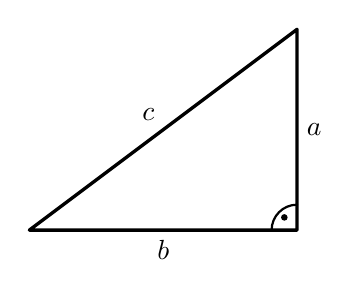
\begin{tikzpicture}[scale=0.85,line cap=round,line join=round]
  \coordinate (A) at (0,0);
  \coordinate (B) at (4,0);
  \coordinate (C) at (4,3);

  \draw[very thick] (A) -- (B) -- (C) -- cycle;
  \draw[thick] (4,0.38) arc[start angle=90,end angle=180,radius=0.38];
  \fill (3.81,0.19) circle (1.4pt);

  \node[below] at (2,0) {$b$};
  \node[right] at (4,1.5) {$a$};
  \node at (1.78,1.72) {$c$};
\end{tikzpicture}

  \end{center}

  \begin{ClozeArea}[\linewidth]{4.5cm}
    \begin{align*}
      c^2&=a^2+b^2,\\
      a&=\sqrt{c^2-b^2}
        =\sqrt{(5\,\mathrm{cm})^2-(4\,\mathrm{cm})^2}\\
       &=\sqrt{9\,\mathrm{cm}^2}=3\,\mathrm{cm}.
    \end{align*}
  \end{ClozeArea}

  Die negative Lösung wird verworfen, da eine Seitenlänge positiv ist.
\end{ExampleBox}
